\chapter{ArchiMate}
\section{Introduccción}
Una arquitectura empresarial generalmente se desarrolla porque las personas clave tienen inquietudes que deben ser abordadas por el negocio y los sistemas de TI dentro de una organización. A esas personas se les conoce comúnmente como "partes interesadas"(stakeholders) de la arquitectura empresarial. El rol del arquitecto es abordar estas inquietudes identificando y refinando la motivación y las estrategias expresadas por las partes interesadas y según estas estrategias desarrollar los  diagramas de arquitectura que muestren cómo aborda y equilibrar las inquietudes de los interesados. Sin una arquitectura empresarial, es poco probable que se tengan en cuenta todas las inquietudes y requisitos \cite{ArchiMate1.0}. 

El lenguaje de modelado de Arquitectura ArchiMate proporciona una representación uniforme de diagramas que describen arquitecturas empresariales. Incluye conceptos para especificar arquitecturas interrelacionadas, puntos de vista específicos para partes interesadas seleccionadas y mecanismos de personalización del lenguaje. Ofrece un enfoque arquitectónico integrado que describe, visualiza y muestra diferentes dominios de arquitectura y sus relaciones y dependencias subyacentes. Su framework proporciona un mecanismo de estructuración para dominios de arquitectura, capas y aspectos. Distingue entre los elementos del modelo y su notación, para permitir representaciones variadas y orientadas a las partes interesadas de la información de arquitectura.

\newpage
El lenguaje utiliza la orientación al servicio para distinguir y relacionar las capas empresariales, de aplicaciones y tecnológicas de las arquitecturas empresariales, y utiliza las relaciones de realización para relacionar elementos concretos con elementos más abstractos en estas capas.

ArchiMate es un lenguaje ligero y escalable en varios aspectos:

\begin{itemize}
\item Su marco de arquitectura es simple pero lo suficientemente completo como para proporcionar un buen mecanismo de estructuración para dominios de arquitectura, capas y aspectos.

\item El lenguaje incorpora pensamientos modernos del paradigma de orientación al servicio que promueve un nuevo principio de organización en términos de servicios (comerciales, de aplicaciones e infraestructura) para las organizaciones, con consecuencias de largo alcance para su arquitectura empresarial.

\item Aunque se parece intencionalmente al lenguaje de modelado unificado (UML), la notación de modelado ArchiMate es intuitiva y mucho más ligera que la propuesta por UML 2.0. Sin embargo el lenguaje es lo suficientemente expresivo como para permitir el modelado de todas las capas (infraestructura comercial, de aplicaciones y de tecnología) y todos los aspectos (estructura, comportamiento e información) de una organización de manera integrada.

\item Los dos estándares de arquitectura empresarial de The Open Group, TOGAF y ArchiMate, se complementan entre sí y se pueden usar bien en combinación\cite{ArchiMate2.0}.
\end{itemize}
\newpage

\section{Definiciones}

\begin{itemize}
\item  \textbf{\textit{Empresa:}} El término empresa en el contexto de arquitectura empresarial se puede utilizar para denotar tanto un toda la empresa, que abarca todos sus sistemas de información y un dominio específico dentro del empresa.

\item \textbf{\textit{Arquitectura:}}Una descripción formal de un sistema, o un plan detallado del sistema a nivel de componente para guiar su implementación.

\item \textbf{\textit{ArchiMate Core Framework:}}Estructura para clasificar lo elementos de Archimate la cúal consta tiene tres capas y tres aspectos.

\item \textbf{\textit{Lenguaje central de ArchiMate:}}Define el concepto y las relaciones del modelo empresarial. Estos conceptos están incluidos en tres capas: Negocio, Aplicación, y Tecnología.

\item \textbf{\textit{Lenguaje central de ArchiMate:}}Define el concepto y las relaciones del modelo empresarial. Estos conceptos están incluidos en tres capas: Negocio, Aplicación, y Tecnología.

\item \textbf{\textit{Aspecto:}}Clasificación de los elementos basada en las características de cada capa.

\item \textbf{\textit{Atributo:}}Propiedad asociada  a un elemento.

\item \textbf{\textit{Concepto:}}Un elemento o una relación.

\item \textbf{\textit{Conformidad:}}Cumplimiento de los requisitos especificados.

\item \textbf{\textit{Implementación conforme:}}Implementación que satisface los requisitos de conformidad definidos.

\item \textbf{\textit{Elemento:}}Unidad básica.

\item \textbf{\textit{Elemento central:}}Una estructura o elemento de comportamiento en una de las capas centrales del lenguaje.

\item \textbf{\textit{Elemento Compuesto:}}Un elemento compuesto de otros elementos o capas del lenguaje.

\item \textbf{\textit{Capa:}}Una abstracción del marco archimate en el que se puede modelar una empresa.

\item \textbf{\textit{Modelo:}}Colección de conceptos en la estructura del lenguaje.

\item \textbf{\textit{Relación:}}Conexión entre un concepto de origen y destino..

\end{itemize}

\section{Propuesta de diseño}
Un desafío clave en el desarrollo de un metamodelo general para la arquitectura empresarial es lograr un equilibrio entre la especificidad de los lenguajes para dominios de arquitectura individuales y un conjunto muy general de conceptos de arquitectura, que refleja una visión de los sistemas como un mero conjunto de entidades interrelacionadas.\cite{ArchiMate2.1}.

\begin{figure}[h!]
	\centering
	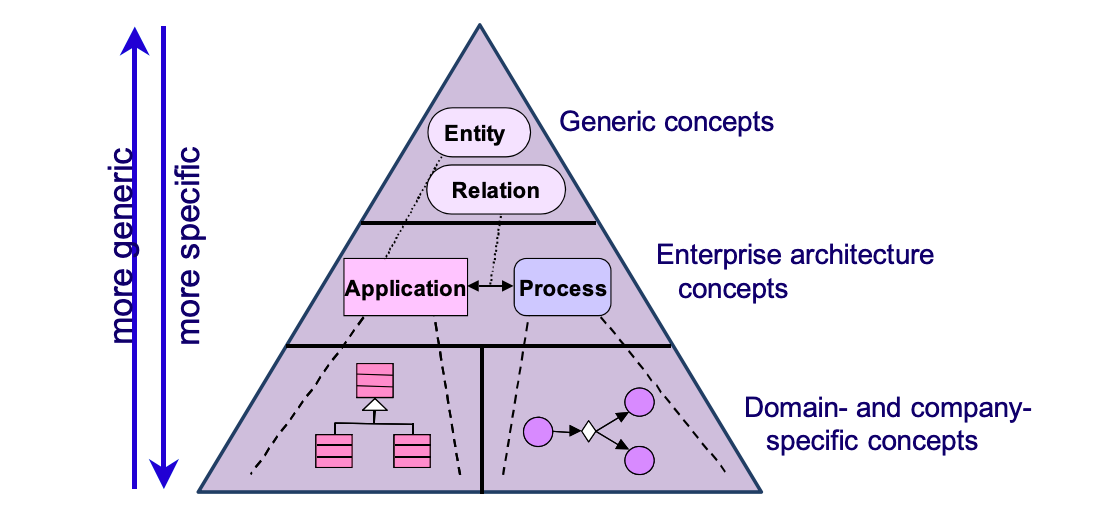
\includegraphics[width=1\linewidth]{ARQUITECTURA/imgs/design}
	\caption{Metamodelos en diferentes niveles de especificación}
	\label{design}
\end{figure}
En la base del triángulo de la figura \ref{design} encontramos los metamodelos de los conceptos de modelado de arquitectura utilizados por organizaciones específicas, así como una variedad de lenguajes y estándares existentes; UML es un ejemplo de un lenguaje en esta categoría. En el triángulo encontramos el metamodelo más usualmente para arquitecturas de sistemas, esencialmente un metamodelo que comprende nociones simplemente como entidad y relación. El diseño del lenguaje ArchiMate comenzó a partir de un conjunto de conceptos relativamente genéricos (Se observan en el cúspide de la piramide) orientados a aplicaciones especializadas en diferentes capas arquitectónicas, La restricción de diseño más importante en el lenguaje es que ha sido diseñado explícitamente para ser lo más sencillo  posible, pero aún utilizable para la mayoría de las tareas de modelado  de la arquitectura empresarial. Muchos otros lenguajes, como UML 2.0, intentan satisfacer todas las necesidades de todos los usuarios posibles. ArchiMate se ha limitado a los conceptos que son suficientes para realizar un modelo de manera practica.
\newpage
\section{Lenguaje Central}
El lenguaje central consta de tres tipos principales de elementos : elementos de estructura activa, comportamiento , y elementos de estructura pasiva (objetos).En la figura \ref{central} se puede visualizar la estructura central de Archimate\cite{ArchiMate3.0}.

\begin{figure}[h!]
	\centering
	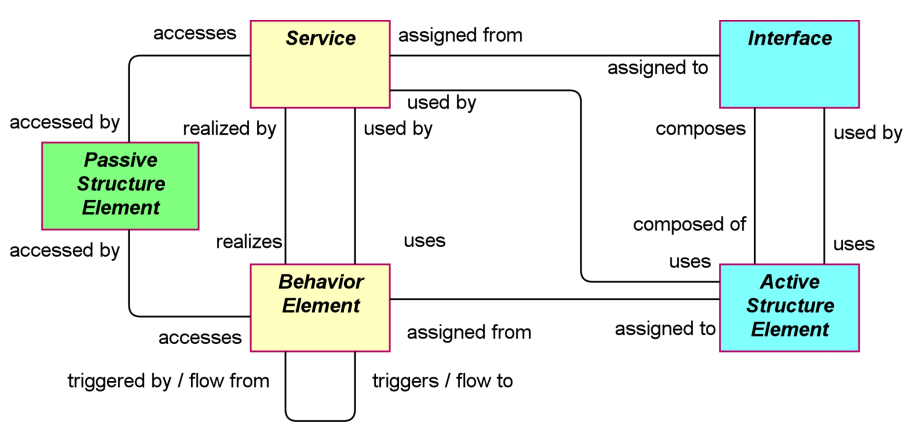
\includegraphics[width=1\linewidth]{ARQUITECTURA/imgs/central}
	\caption{Lenguaje Central de Archimate}
	\label{central}
\end{figure}

\begin{itemize}
	
	\item  \textbf{\textit{Elemento de estructura activa:}}se define como una entidad que es capaz de realizar comportamientos.
	
	\item  \textbf{\textit{Elemento de comportamiento:}} se define como una unidad de actividad realizada por una o más estructuras de elementos activos.
	
	\item  \textbf{\textit{Elemento de estructura pasiva:}} se define como un objeto en el que se realiza el comportamiento.
	
	\item  \textbf{\textit{Servicio:}} se define como una unidad de funcionalidad que un sistema expone a su entorno.
	
	\item  \textbf{\textit{Interfaz:}} se define como un punto de acceso donde uno o más servicios están disponibles para el entorno.
	
\end{itemize}
\newpage
\section{Estructura del Lenguaje}
La especificación y descripción inequívocas de los componentes de la arquitectura empresarial y especialmente de sus relaciones requieren un lenguaje de modelado de arquitectura que aborde el problema de la alineación consistente y facilite un modelado coherente de las arquitecturas empresariales. Un desafío clave en el desarrollo de un meta modelo general para Arquitectura Empresarial es lograr un equilibrio entre la especificidad de los lenguajes para dominios de arquitectura individuales y un conjunto muy general de conceptos de arquitectura, que refleja una visión de los sistemas como un mero conjunto de entidades.

El diseño del lenguaje ArchiMate comenzó a partir de un conjunto de conceptos relativamente genéricos. 
La ventaja mas importante del diseño de el lenguaje es que ha sido diseñado explícitamente para ser utilizado para la mayoría de las tareas de modelado de arquitectura empresarial. La Figura \ref{altonivel} describe la estructura jerárquica de nivel superior del lenguaje:
\begin{figure}[h!]
	\centering
	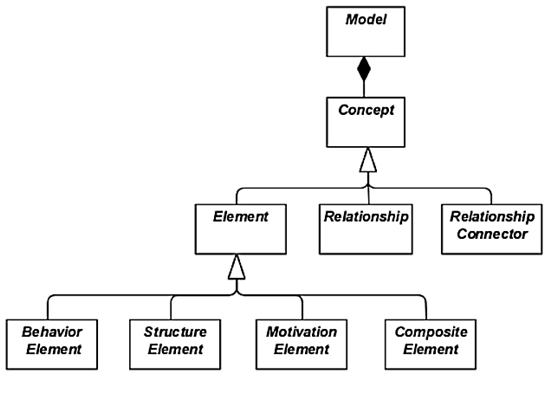
\includegraphics[width=1\linewidth]{ARQUITECTURA/imgs/altonivel}
	\caption{Jerarquía de nivel superior de los conceptos de ArchiMate}
	\label{altonivel}
\end{figure}

\newpage
\subsubsection{Colaboración e interacción}
Al profundizar en la estructura del lenguaje, distinguimos entre el comportamiento realizado por un solo elemento de estructura (por ejemplo, actor, componente de rol, etc.) o el comportamiento colectivo (interacción) que se realiza mediante una colaboración de elementos con múltiple estructura. En la figura \ref{comportamiento} se observa la relación entre la Colaboración y la Interacción.

\begin{figure}[h!]
	\centering
	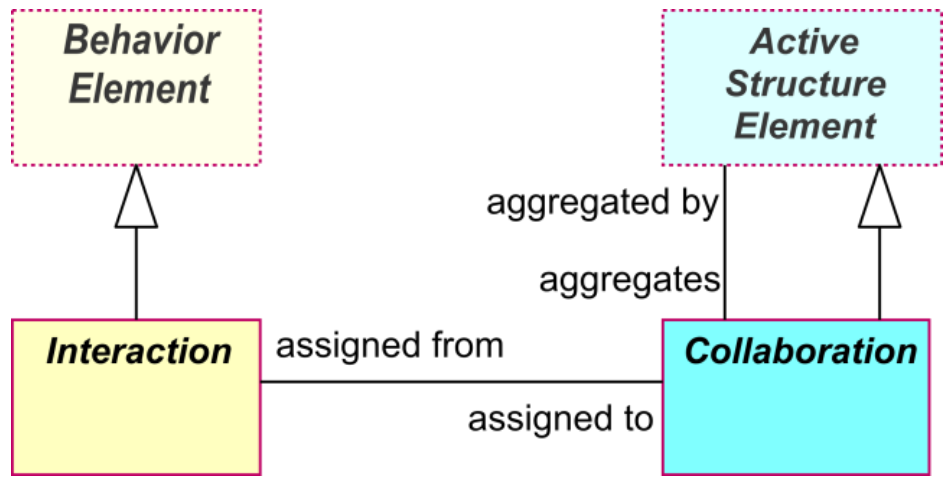
\includegraphics[width=0.9\linewidth]{ARQUITECTURA/imgs/comportamiento}
	\caption{Colaboración e Interacción}
	\label{comportamiento}
\end{figure}

\begin{itemize}
\item \textbf{\textit{Colaboración}} se define como una agrupación temporal de dos o más elementos de estructura, trabajando juntos para realizar un comportamiento colectivo.Este comportamiento colectivo puede modelarse como una interacción.

\item \textbf{\textit{Interacción}} se define como una unidad de comportamiento realizada por una colaboración de dos o más elementos de estructura.
\end{itemize}

\subsubsection{Relaciones}
ArchiMate contiene un conjunto central de relaciones. Varias de estas relaciones se han adoptado de los conceptos de relación correspondientes que se producen en los estándares existentes; Por ejemplo, las relaciones: tales como composición, agregación, asociación y especialización se toman de UML 2.0, mientras que la activación se usa en muchos lenguajes de modelado de procesos de negocios.

\newpage

\subsubsection{Capas}
El lenguaje central de ArchiMate define una estructura de elementos genéricos y sus relaciones, que pueden caracterizarse en tres capas se definen dentro del lenguaje central de ArchiMate de la siguiente manera:

\begin{enumerate}
\item La \textbf{\textit{capa empresarial}} representa los servicios  ofrecidos a los clientes, que se realizan en la organización mediante procesos empresariales realizados por actores empresariales.

\item La \textbf{\textit{capa de aplicación}} muestra los servicios de  que respaldan el negocio y las aplicaciones que los realizan.

\item La \textbf{\textit{capa de tecnología}} muestra los servicios de procesamiento, almacenamiento y comunicación necesarios para ejecutar las aplicaciones, el hardware de la computadora,la comunicación y el software del sistema que realizan dichos servicios. Se agregan elementos físicos para modelar equipos físicos, materiales y redes de distribución para esta capa
\end{enumerate}

\subsubsection{Aspectos}
Los aspectos estan definidos por los tres tipos de elementos 
\begin{enumerate}
\item El \textbf{\textit{aspecto de estructura activa}}  representa los conceptos estructurales,los actores empresariales, los componentes de la aplicación y los dispositivos que muestran un comportamiento real; es decir, los sujetos de la actividad.
\item El \textbf{\textit{aspecto de comportamiento}} representa el comportamiento (procesos, funciones, eventos y servicios) realizados por los actores. 
\item El \textbf{\textit{aspecto de estructura pasiva}} representa los objetos en los que se realiza el comportamiento. Generalmente son objetos de información en la capa empresarial y objetos de datos en la capa de aplicación, pero también pueden usarse para representar objetos físicos.
\end{enumerate}

\newpage
\subsubsection{Framework de ArchiMate}
Los aspectos del core y las  capas identificados en las secciones anteriores se pueden organizar como un framework de nueve celdas, como se ilustra en la Figura \ref{core}. Es importante entender que la clasificación de conceptos basada en aspectos y capas es solo global. Es imposible definir un límite estricto entre los aspectos y las capas, porque los conceptos que los vinculan juegan un papel central en una descripción arquitectónica coherente\cite{ArchiMate3.0.1}.

\begin{figure}[h!]
	\centering
	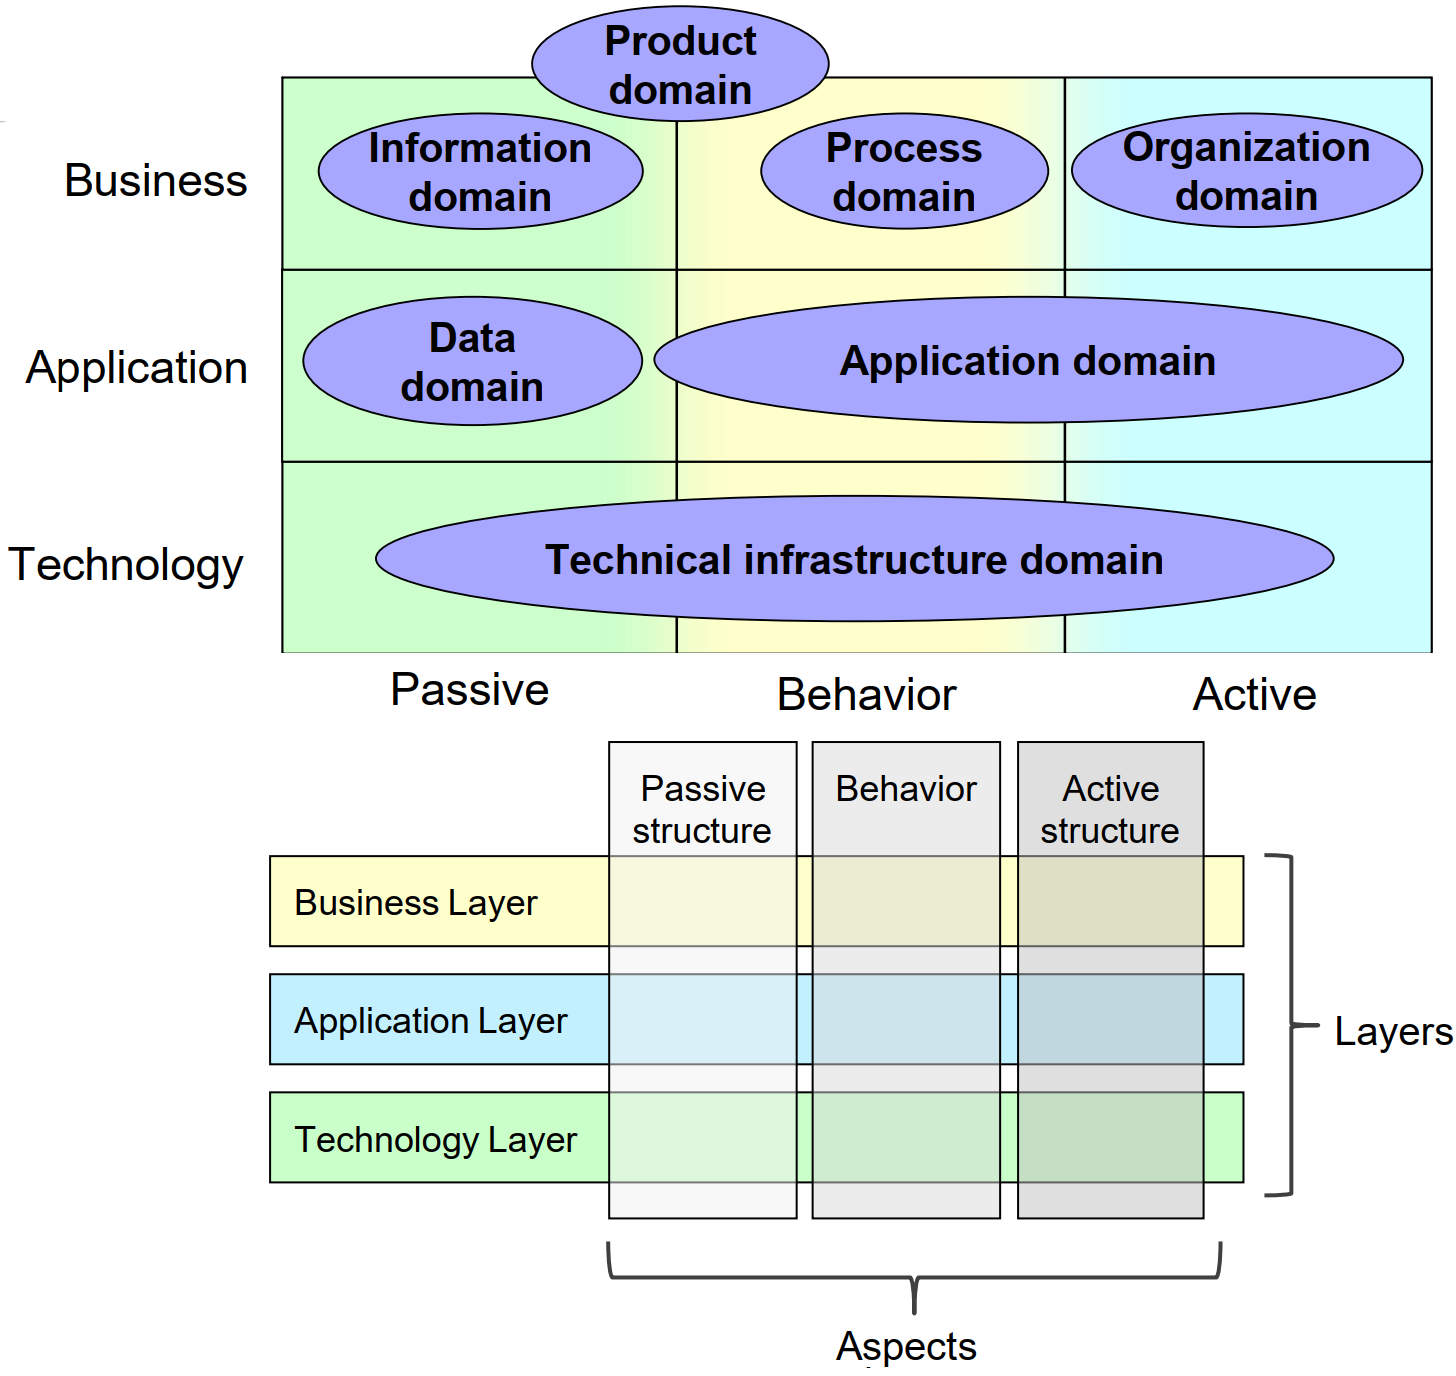
\includegraphics[width=1\linewidth]{ARQUITECTURA/imgs/core}
	\caption{Core del Framework de ArchiMate}
	\label{core}
\end{figure}


La estructura del Framework permite modelar la empresa desde diferentes puntos de vista, donde la posición dentro de las celdas resalta las inquietudes del interesado.

\newpage
El lenguaje completo de ArchiMate, como se describe en la versión actual del estándar, agrega una serie de capas y un aspecto al Framework.La capa fisica,la capa de implementación y migración, y el aspecto de motivación.Estos elementos adicionales se describen a continuación: 

\begin{enumerate}
	\item La \textbf{\textit{capa fisica}}  representa los elementos físicos que modelan instalaciones,equipos y redes de distribución y materiales.
	\item La \textbf{\textit{capa de implementación y migración}} representa los conceptos para soportar las últimas fases de ADM, relacionadas con la implementación y migración de arquitecturas:Oportunidades y soluciones, Planificación de la migración y Gobierno de la implementación. 
	\item El \textbf{\textit{aspecto de motivación}} representa los  objetivos, principios y requerimientos que se alinean con la razón subyacente a la arquitectura de una empresa.
\end{enumerate}
En la Figura \ref{marco} se muestra el framework completo de ArchiMate con los aspectos y capas adicionales.

\begin{figure}[h!]
	\centering
	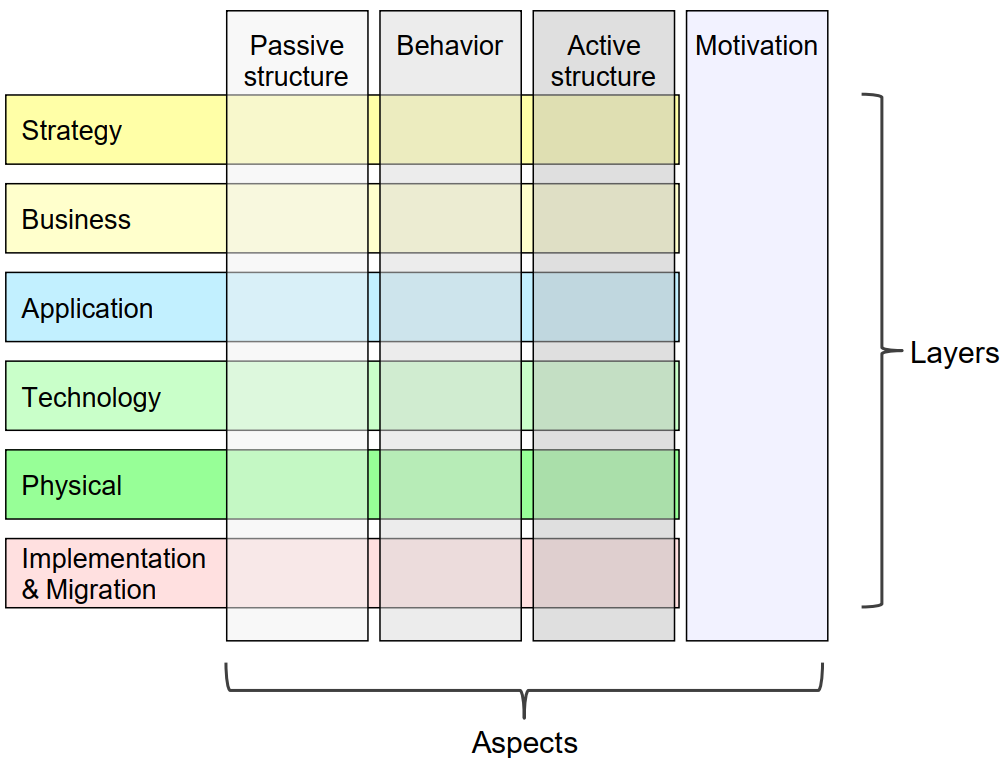
\includegraphics[width=0.8\linewidth]{ARQUITECTURA/imgs/marco}
	\caption{Framework completo de ArchiMate}
	\label{marco}
\end{figure}

\section{ArchiMate y TOGAF}
TOGAF es un framework de arquitectura, un conjunto de métodos y herramientas para desarrollar una amplia gama de diferentes arquitecturas de TI. Permite a los usuarios de TI diseñar, evaluar y construir la arquitectura adecuada para su organización, y reduce los costos de planificación, diseño implementando arquitecturas basadas en soluciones de sistemas abiertos. La clave de TOGAF es el Método de Desarrollo de Arquitectura (ADM), un método confiable para desarrollar una arquitectura empresarial de TI que satisfaga las necesidades de su negocio.

El framework de TOGAF considera una arquitectura empresarial global compuesta de un conjunto de arquitecturas estrechamente interrelacionadas: arquitectura empresarial, arquitectura de sistemas de información (que comprende arquitectura de datos y arquitectura de aplicaciones) y arquitectura tecnológica (TI). El lenguaje ArchiMate, como se describe en la especificación 1.0, complementa TOGAF en el sentido de que proporciona un conjunto de conceptos independientes del proveedor, incluida una representación gráfica, que ayuda a crear un modelo coherente e integrado, que puede representarse en la forma gráfica de TOGAF. La estructura del lenguaje ArchiMate corresponde perfectamente con las tres arquitecturas principales como se aborda en el TOGAF ADM. Esta compatibilidad  genera una relación entre los diagramas de TOGAF y diagramas de ArchiMate.

Sin embargo, algunas vistas de TOGAF no coinciden en el núcleo de ArchiMate. Parcialmente, esto se debe a que el alcance de TOGAF es más amplio y, en particular, aborda más de los problemas estratégicos de alto nivel y los aspectos de ingeniería de nivel inferior del desarrollo del sistema, mientras que ArchiMate core se limita al nivel de abstracción de la arquitectura empresarial.

Aunque algunos de los enfoques que se definen en TOGAF no pueden asignarse fácilmente a los enfoques de ArchiMate, ArchiMate y sus técnicas de análisis admiten los conceptos abordados. Si bien no existe una correspondencia uno a uno entre ellos, todavía hay una buena cantidad de acomple entre ellos. Aunque los enfoques correspondientes de ArchiMate y TOGAF no necesariamente tienen una cobertura idéntica, podemos ver que muchos enfoques de ambos métodos abordan en gran medida los mismos problemas. TOGAF y ArchiMate pueden usarse fácilmente en conjunto y parecen cubrir gran parte del mismo terreno, aunque con algunas diferencias en alcance.

La estructura del lenguaje central de ArchiMate se corresponde estrechamente con las tres arquitecturas principales que se abordan en el TOGAF ADM. Esto se ilustra en la Figura \ref{togaf}.
\begin{figure}[h!]
	\centering
	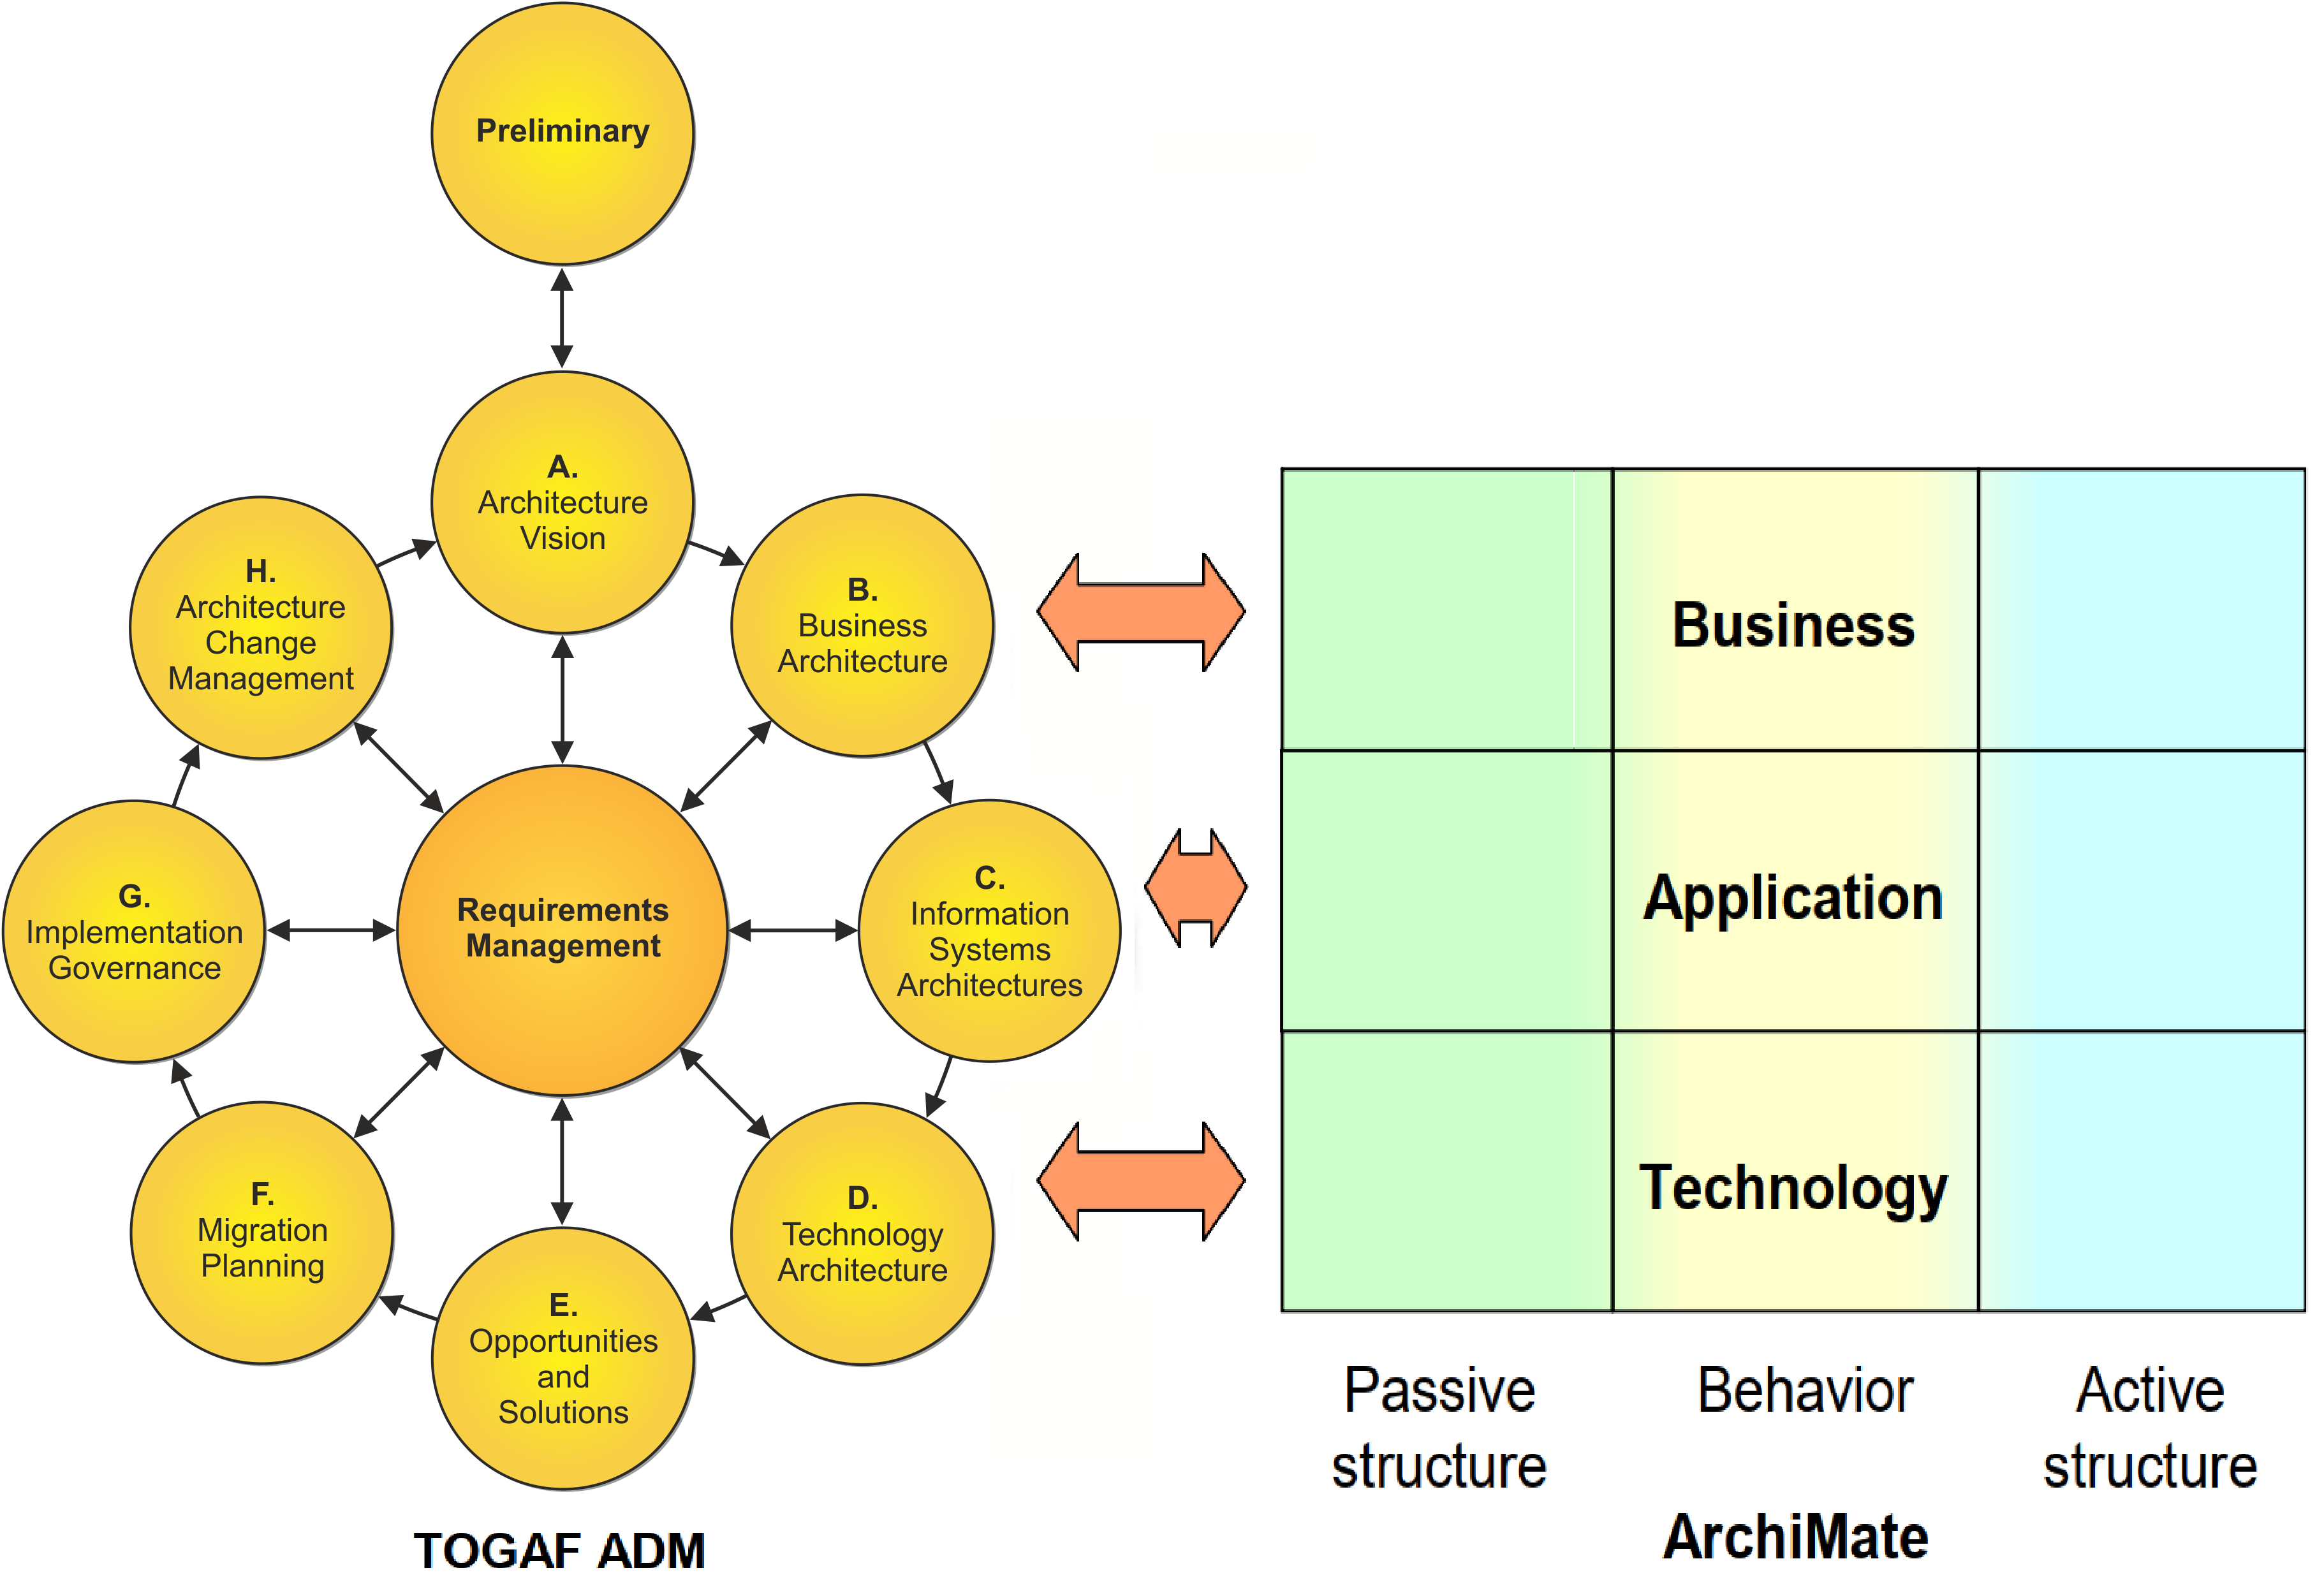
\includegraphics[width=1\linewidth]{ARQUITECTURA/imgs/togaf}
	\caption{Compatibilidad entre Archimate y TOGAF}
	\label{togaf}
\end{figure}
